\chapter{Hajautustaulu}

Tämän luvun tavoitteemme on luoda tietorakenne,
jonka avulla voimme pitää yllä tehokkaasti alkioiden joukkoa,
jossa on seuraavat operaatiot:

\begin{itemize}
\item lisää alkio $x$ joukkoon
\item tarkista, onko alkio $x$ joukossa
\item poista alkio $x$ joukosta
\end{itemize}

Jos alkiot olisivat aina kokonaislukuja
välillä $0,1,\ldots,n-1$, voisimme ratkaista tehtävän
helposti luomalla $n$-kokoisen taulukon, jonka
jokaisessa kohdassa $x$ on luku 0 ($x$ ei ole taulukossa)
tai luku 1 ($x$ on taulukossa).
Tällaisen taulukon avulla voisimme toteuttaa
helposti kaikki yllä olevat operaatiot $O(1)$-ajassa
päivittämällä tai tutkimalla yhtä kohtaa taulukosta.

Tässä luvussa keskitymme kuitenkin yleisempään tilanteeseen,
jossa alkiot eivät ole välttämättä sopivan pieniä kokonaislukuja
vaan ne voivat olla minkä tahansa tyyppisiä, esimerkiksi merkkijonoja.
Osoittautuu, että voimme yleistää yllä olevan idean toteuttamalla
hajautustaulun, jossa jokaisen alkion sijainnin määrää sen hajautusarvo,
ja pystymme edelleen toteuttamaan kaikki operaatiot
tehokkaasti keskimäärin $O(1)$-aikaisesti.

\section{Hajautustaulun toteuttaminen}

\emph{Hajautustaulu} on $n$-kokoinen taulukko,
joka pitää yllä alkioiden joukkoa.
Jokaisessa hajautustaulun kohdassa on lista,
jossa on jokin määrä alkioita.
Jotta voimme käyttää hajautustaulua,
meillä täytyy olla myös \emph{hajautusfunktio},
jonka avulla voimme laskea mille tahansa alkiolle
\emph{hajautusarvon} eli kohdan, johon alkio
tallennetaan hajautustaulussa.

\begin{figure}
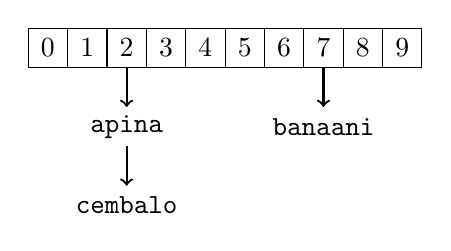
\begin{tikzpicture}[scale=0.5]
\draw (0,0) grid (10,1);
\foreach \x in {0,1,...,9} \node at (0.5+\x,0.5) {\x};
\draw[->,thick] (2.5,0) -- (2.5,-1);
\draw[->,thick] (7.5,0) -- (7.5,-1);
\draw[->,thick] (2.5,-2) -- (2.5,-3);
\node at (2.5,-1.5) {\texttt{apina}};
\node at (7.5,-1.5) {\texttt{banaani}};
\node at (2.5,-3.5) {\texttt{cembalo}};
\end{tikzpicture}
\caption{Hajautustaulu, joka vastaa joukkoa $\{\texttt{apina},\texttt{banaani},\texttt{cembalo}\}$.
Merkkijonojen \texttt{apina} ja \texttt{cembalo} hajautusarvo on 2, ja merkkijonon
\texttt{banaani} hajautusarvo on 7.}
\label{fig:hajtau}
\end{figure}

Kuvassa \ref{fig:hajtau} on esimerkkinä hajautustaulu, jossa on
merkkijonot \texttt{apina}, \texttt{banaani} ja \texttt{cembalo}.
Tässä hajautustaulussa on kymmenen mahdollista kohtaa
($0,1,\ldots,9$), joihin voi tallentaa alkioita listaan.
Merkkijonojen \texttt{apina} ja \texttt{cembalo}
hajautusarvo on 2, joten ne ovat samassa listassa kohdassa 2.
Merkkijonon \texttt{banaani} hajautusarvo taas on 7,
joten se on yksin omassa listassaan.
Kaikki muut hajautustaulun listat ovat tällä hetkellä tyhjiä.

Kun olemme luoneet hajautustaulun, voimme tarkistaa,
onko tietty alkio joukossa, laskemalla sen hajautusarvon
ja käymällä läpi vastaavan listan.
Vastaavasti voimme lisätä alkion joukkoon
lisäämällä sen vastaavan listan loppuun ja poistaa
alkion joukosta poistamalla sen listasta.
Näiden operaatioiden aikavaativuus on $O(k)$,
missä $k$ on alkion hajautusarvoa vastaavan listan pituus,
koska meidän täytyy käydä läpi listalla olevat alkiot.
Hajautustaulun tehokkuus riippuukin siitä,
kuinka pitkiä listat ovat.

\subsection{Hajautusfunktio}

Hajautusfunktio määrittää, mihin kohtaan hajautustaulua
alkio sijoitetaan.
Sen täytyy antaa jokaiselle mahdolliselle alkiolle
hajautusarvo eli kokonaisluku väliltä $0 \dots n-1$,
missä $n$ on hajautustaulun koko.
Muuten meillä on vapaat kädet hajautusfunktion suunnitteluun:
ainoa välttämätön vaatimus on, että tietty alkio saa aina
saman hajautusarvon, jotta voimme löytää sen uudelleen
hajautustaulusta.

Jotta hajautustaulu olisi käyttökelpoinen, hajautusfunktioon
liittyy kuitenkin toinenkin vaatimus:
sen tulisi jakaa alkiot mahdollisimman \emph{tasaisesti}
eri puolille hajautustaulua.
Syynä tähän on, että hajautustaulun tehokkuus riippuu siitä,
miten tasaisesti alkiot ovat jakautuneet.
Jos alkiot ovat jakautuneet tasaisesti ja listat ovat lyhyitä,
voimme lisätä, etsiä ja poistaa alkioita tehokkaasti.

\begin{figure}
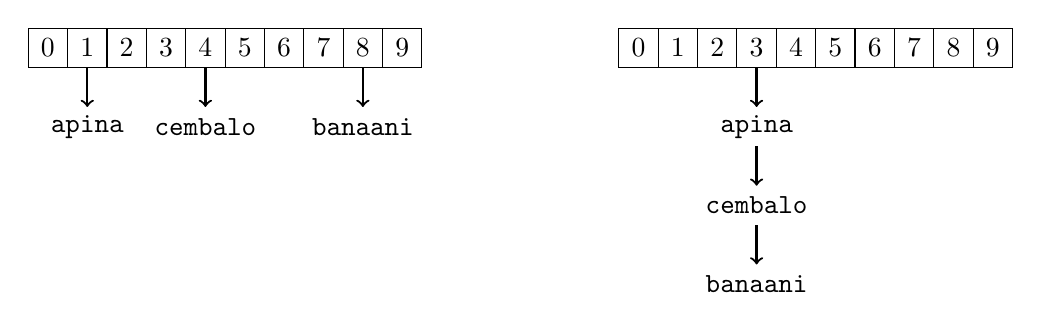
\begin{tikzpicture}[scale=0.5]
\begin{scope}
\draw (0,0) grid (10,1);
\foreach \x in {0,1,...,9} \node at (0.5+\x,0.5) {\x};
\draw[->,thick] (1.5,0) -- (1.5,-1);
\draw[->,thick] (4.5,0) -- (4.5,-1);
\draw[->,thick] (8.5,0) -- (8.5,-1);
\node at (1.5,-1.5) {\texttt{apina}};
\node at (8.5,-1.5) {\texttt{banaani}};
\node at (4.5,-1.5) {\texttt{cembalo}};
\end{scope}
\begin{scope}[xshift=15cm]
\draw (0,0) grid (10,1);
\foreach \x in {0,1,...,9} \node at (0.5+\x,0.5) {\x};
\draw[->,thick] (3.5,0) -- (3.5,-1);
\draw[->,thick] (3.5,-4) -- (3.5,-5);
\draw[->,thick] (3.5,-2) -- (3.5,-3);
\node at (3.5,-1.5) {\texttt{apina}};
\node at (3.5,-5.5) {\texttt{banaani}};
\node at (3.5,-3.5) {\texttt{cembalo}};
\end{scope}
\end{tikzpicture}
\caption{Kaksi hajautustaulua joukolle $\{\texttt{apina},\texttt{banaani},\texttt{cembalo}\}$.
Vasemmassa taulussa hajautus on onnistunut täydellisesti,
oikeassa taulussa kaikki alkiot ovat samassa listassa.}
\label{fig:hajjak}
\end{figure}

Kuva \ref{fig:hajjak} näyttää kaksi hajautustaulua, jotka vastaavat
samaa joukkoa eri hajautusfunktioilla.
Vasemmassa taulussa hajautus on onnistunut täydellisesti
ja jokainen alkio on omassa listassaan.
Oikeassa taulussa taas kaikki alkiot ovat joutuneet samaan
listaan eikä hajautustaulusta ole mitään hyötyä.
Tavoitteemme on, että saisimme aikaan hajautusfunktion,
jonka toiminta on lähempänä vasenta taulua.

Tarkastelemme seuraavaksi esimerkkinä hajautusfunktioita,
joilla voi laskea hajautusarvoja merkkijonoille.
Käytännössä meidän riittää määritellä hajautusfunktio,
joka muuttaa merkkijonon epänegatiiviseksi kokonaisluvuksi,
koska tämän jälkeen saamme helposti kokonaisluvun
väliltä $0 \dots n-1$ ottamalla alkuperäisestä luvusta jakojäännöksen $n$:llä.

Oletamme, että merkkijonossa on $k$ merkkiä,
joiden merkkikoodit\footnote{Käytämme tässä merkkien ASCII-koodeja.
Esimerkiksi Javassa char-merkin \texttt{c} koodin saa
selville kirjoittamalla \texttt{(int)c}, eli esimerkiksi
\texttt{(int)'a'} on 97.} ovat $c_0,c_1,\dots,c_{k-1}$.
Esimerkiksi jos merkkijono on \texttt{apina},
$k=5$ ja koodit ovat $c_0=97$, $c_1=112$, $c_2=105$,
$c_3=110$ ja $c_4=97$.
Seuraavassa on kolme mahdollista tapaa määritellä hajautusfunktio:

\begin{enumerate}
\item Hajautusarvo on merkkijonon pituus $k$.
Esimerkiksi merkkijonon \texttt{apina} hajautusarvo on 5.
\item Hajautusarvo on merkkikoodien summa
\[ c_0 + c_1 + \dots + c_{k-1}.\]
Merkkijonon \texttt{apina} hajautusarvo on
\[97+112+105+110+97=521.\]
\item Hajautusarvo on painotettu merkkikoodien summa
\[ A^{k-1} c_0 + A^{k-2} c_1 + \dots + A^0 c_{k-1},\]
missä $A$ on sopiva vakio.
Esimerkiksi jos $A=7$, merkkijonon \texttt{apina} hajautusarvo on
\[7^4 \cdot 97+7^3 \cdot 112+7^2 \cdot 105+7^1 \cdot 110+7^0 \cdot 97=61235.\]
\end{enumerate}

Kaikki yllä olevat hajautusfunktiot ovat toimivia,
mutta ne eivät ole yhtä hyviä.
Funktio 1 ei ole kovin hyvä, koska se antaa monelle
usein esiintyvälle merkkijonolle saman hajautusarvon.
Esimerkiksi suomen kielessä on suuri määrä viisikirjaimisia
sanoja ja ne kaikki saavat saman hajautusarvon tätä
hajautusfunktiota käyttämällä.
Funktio 2 on jo parempi, mutta siinä on heikkoutena,
että jos kahdessa merkkijonossa on samat merkit eri
järjestyksessä, ne saavat aina saman hajautusarvon.
Funktio 3 eli \emph{polynominen hajautus} korjaa tämän puutteen
asettamalla summaan painoja, jotka riippuvat merkkien kohdista.
Tämä on käytännössä hyvä tapa määritellä hajautusfunktio,
jota käytetään esimerkiksi Javan standardikirjastossa.

\subsection{Hajautustaulun tehokkuus}

Hajautustaulun tehokkuus riippuu siitä, montako kohtaa
hajautustaulussa on (hajautustaulun koko $n$)
sekä miten tasaisesti hajautusfunktio jakaa alkiota
eri puolelle hajautustaulua.
Jos oletamme, että alkiot jakautuvat tasaisesti
ja hajautustaulussa on yhteensä $m$ alkiota,
jokaiseen listaan osuu noin $m/n$ alkiota
eli hajautustaulun operaatiot toimivat $O(m/n)$-ajassa.
Jos edelleen $n$ on valittu niin suureksi,
että $m/n$ on pieni vakio, voimme ajatella,
että hajautustaulun operaatiot toimivat $O(1)$-ajassa.

Tämän analyysin heikkoutena on, että \emph{oletamme}
hajautusfunktion toimivan hyvin ja jakavan alkioita
tasaisesti hajautustauluun. Entä jos näin ei olekaan?

Hajautustaulun tehokkuus riippuu aina myös siitä,
mitä alkioita sinne laitetaan.
Vaikka olisimme valinneet hajautustaulun koon ja
hajautusfunktion miten huolellisesti tahansa,
ilkeä vastustaja voi kuitenkin valita alkiot
niin, että jokaisen alkion hajautusarvo on sama ja
kaikki menevät samaan listaan hajautustaulussa.
Tällöin hajautustaulun operaatiot vievät aikaa $O(m)$.
Tämä riski on aina olemassa, kun käytämme hajautustaulua.

Onneksi hajautustaulu toimii käytännössä hyvin ja 
uhka siitä, että jokainen tai edes suuri osa alkioista
menisi samaan listaan, on hyvin pieni.

\section{Hajautus Javassa}

Javassa on kaksi hajautustaulua käyttävää tietorakennetta:
\texttt{HashSet} pitää yllä joukkoa alkioista
ja \texttt{HashMap} on yleistetty taulukko,
jossa on joukko avain-arvo-pareja.
Seuraavaksi tutustumme tarkemmin näihin rakenteisiin.

\subsection{\texttt{HashSet}}

Javan \texttt{HashSet}-rakenne pitää yllä joukkoa alkioista
hajautustaulun avulla.
Rakenteen tärkeimmät operaatiot ovat seuraavat:

\begin{itemize}
\item $\texttt{add}(x)$: lisää alkio $x$ joukkoon
\item $\texttt{contains}(x)$: tarkasta, onko alkio $x$ joukossa
\item $\texttt{remove}(x)$: poista alkio $x$ joukosta
\item $\texttt{size}()$: laske, montako alkiota on joukossa
\end{itemize}

Esimerkiksi seuraava koodi luo joukon, jossa voi olla
kokonaislukuja, ja lisää luvut 3, 5 ja 8 joukkoon.
Tämän jälkeen koodi tulostaa joukon sisällön.

\begin{code}
HashSet<Integer> joukko = new HashSet<Integer>();
joukko.add(3);
joukko.add(5);
joukko.add(8);
System.out.println(joukko); // [3, 5, 8]
\end{code}

Huomaa, että jokainen alkio voi esiintyä vain kerran joukossa.
Esimerkiksi vaikka seuraava koodi lisää luvun 5 kolmesti
joukkoon, se menee sinne vain ensimmäisellä kerralla ja
muut lisäykset jätetään huomiotta.

\begin{code}
HashSet<Integer> joukko = new HashSet<Integer>();
joukko.add(5);
joukko.add(5);
joukko.add(5);
System.out.println(joukko); // [5]
\end{code}

Olennainen seikka \texttt{HashSet}-rakenteessa on,
että operaatiot \texttt{add}, \texttt{contains} ja \texttt{remove}
toimivat kaikki keskimäärin tehokkaasti ajassa $O(1)$
hajautustaulun ansiosta.
Niinpä voimme tehdä mitä tahansa muutoksia ja hakuja
rakenteeseen ja koodi toimii nopeasti.
Tämä ei olisi mahdollista \texttt{ArrayList}-rakenteessa,
jossa operaatiot \texttt{contains} ja \texttt{remove}
vievät aikaa $O(n)$.

\subsection{\texttt{HashMap}}

\texttt{HashMap}-rakenne pitää yllä joukkoa avain-arvo-pareja.
Rakennetta voi ajatella taulukon yleistyksenä:
$n$ alkion taulukossa avaimet ovat aina kokonaisluvut
$0,1,\ldots,n-1$, mutta \texttt{HashMap} sallii
avaimina minkä tahansa tyyppisiä alkioita eikä niiden
tarvitse olla peräkkäisiä kokonaislukuja.

Esimerkiksi seuraava koodi luo sanakirjan, jossa sekä
avaimet että arvot ovat merkkijonoja.
Sanakirjaan voi syöttää merkkijonopareja, jotka kertovat
sanan käännöksen suomesta englanniksi.
Metodi \texttt{put} lisää uuden avain-arvo-parin,
ja metodi \texttt{get} hakee arvon avaimen perusteella.

\begin{code}
HashMap<String,String> sanakirja = new HashMap<String,String>();

sanakirja.put("apina","monkey");
sanakirja.put("banaani","banana");
sanakirja.put("cembalo","harpsichord");

System.out.println(sanakirja.get("banaani")); // banana
\end{code}

Hyödyllinen on myös metodi \texttt{containsKey},
jonka avulla voi tarkastaa, onko tietylle avaimelle
tallennettu arvoa:

\begin{code}
if (sanakirja.containsKey(sana)) {
    System.out.println("Käännös: " + sanakirja.get(sana));
} else {
    System.out.println("Sana puuttuu sanakirjasta!");
}
\end{code}

Koska \texttt{HashMap} on toteutettu hajautustaulun avulla,
sen operaatiot toimivat tehokkaasti keskimäärin $O(1)$-ajassa.

\subsection{Metodi \texttt{hashCode}}

Javan hajautustaulut perustuvat siihen, että olioissa
on metodi \texttt{hashCode}, jonka avulla olio kertoo
pyydettäessä hajautusarvonsa.
Voimme esimerkiksi selvittää merkkijonon \texttt{ABC}
hajautusarvon näin:

\begin{code}
System.out.println("ABC".hashCode());
\end{code}

Tämä koodi tulostaa luvun 64578,
joka on siis merkkijonon \texttt{ABC} hajautusarvo Javassa.

Metodi \texttt{hashCode} on toteutettu valmiiksi Javan
sisäisiin tyyppeihin, kuten \texttt{Integer} ja \texttt{String},
joten voimme käyttää niitä suoraan hajautustauluissa.
Kuitenkin jos meillä on itse tehty luokka, jonka olioita
haluamme käyttää hajautustauluissa, meidän on toteutettava
itse metodi \texttt{hashCode}.

Esimerkiksi jos meillä on luokka \texttt{Asiakas},
jossa on kenttinä merkkijonot
\texttt{etunimi} ja \texttt{sukunimi},
voisimme toteuttaa metodin \texttt{hashCode} seuraavasti:

\begin{code}
public class Asiakas {
    private String etunimi;
    private String sukunimi;

    int hashCode() {
        return etunimi.hashCode()+sukunimi.hashCode();
    }

    // ...
}
\end{code}
